% answers.tex —— 2000 年·上海卷·文科 · 参考答案与详细解析片段
% 由 tools/generate_projects.py 依来源总账自 2000/2000_数学真题_上海文_试题.md + 2000/2000_数学真题_上海文_解析正文.md + 2000/2000_数学真题_上海文_答案要点.md 生成，勿手改（改源 MD 后重跑）


\begin{gktip}
\textbf{来源说明}：固定 PDF 只有题面，没有答案、解析或评分页。以下为本库独立推导，不是官方解析；出版物版本、复制链及官方身份未核，\texttt{paper_id=gk-2000-regular-shanghai-arts}、\texttt{official_answer=null}。Q21 固定题面的指数与同期答案副本冲突，相关分支均保留条件性标注。
\end{gktip}

\gkpart{一、填空题}

\begin{answer}
\gksolhead{1}{}

\textbf{题目}：

已知向量 $\overrightarrow{OA}=(-1,2)$、$\overrightarrow{OB}=(3,m)$，若 $\overrightarrow{OA}\perp\overrightarrow{OB}$，则 $m=\underline{\qquad}$。

\Needspace{4\baselineskip}
\textbf{解析}

\Needspace{5\baselineskip}
垂直向量的数量积为零，因此

\nopagebreak[4]
\[
(-1,2)\cdot(3,m)=-3+2m=0,
\]

解得 $m=\dfrac32$。

\gkanswer{答案：$m=\dfrac{3}{2}$}

\end{answer}
\begin{answer}
\gksolhead{2}{}

\textbf{题目}：

函数 $y=\log_{2}\dfrac{2x-1}{3-x}$ 的定义域为 $\underline{\qquad}$。

\Needspace{4\baselineskip}
\textbf{解析}

\Needspace{5\baselineskip}
对数真数须为正，故

\nopagebreak[4]
\[
\frac{2x-1}{3-x}>0.
\]

\Needspace{5\baselineskip}
临界点为 $\dfrac12$ 与 $3$。按区间作符号判断，分式在两临界点之间为正，因此定义域为

\nopagebreak[4]
\[
\left(\frac12,3\right).
\]

\gkanswer{答案：$\left(\dfrac{1}{2},3\right)$}

\end{answer}
\begin{answer}
\gksolhead{3}{}

\textbf{题目}：

圆锥曲线 $\dfrac{(x-1)^2}{16}-\dfrac{y^2}{9}=1$ 的焦点坐标是 $\underline{\qquad}$。

\Needspace{4\baselineskip}
\textbf{解析}

\Needspace{5\baselineskip}
双曲线中心为 $(1,0)$，且 $a^2=16$、$b^2=9$。于是

\nopagebreak[4]
\[
c^2=a^2+b^2=25,\qquad c=5.
\]

实轴沿 $x$ 轴，焦点为 $(1\pm5,0)$，即 $(-4,0)$、$(6,0)$。

\gkanswer{答案：$(-4,0)$、$(6,0)$}

\end{answer}
\begin{answer}
\gksolhead{4}{}

\textbf{题目}：

计算：$\displaystyle\lim_{n\to\infty}\left(\dfrac{n}{n+2}\right)^n=\underline{\qquad}$。

\Needspace{4\baselineskip}
\textbf{解析}

\nopagebreak[4]
\[
\left(\frac{n}{n+2}\right)^n
=\left(1+\frac2n\right)^{-n}.
\]

利用 $\lim_{n\to\infty}(1+\frac2n)^n=e^2$，所求极限为 $e^{-2}$。

\gkanswer{答案：$e^{-2}$}

\end{answer}
\begin{answer}
\gksolhead{5}{}

\textbf{题目}：

已知 $f(x)=2^x+b$ 的反函数为 $f^{-1}(x)$，若 $y=f^{-1}(x)$ 的图象经过点 $Q(5,2)$，则 $b=\underline{\qquad}$。

\Needspace{4\baselineskip}
\textbf{解析}

\Needspace{5\baselineskip}
反函数图象经过 $(5,2)$，等价于原函数图象经过交换坐标后的点 $(2,5)$，即 $f(2)=5$。代入 $f(x)=2^x+b$，得

\nopagebreak[4]
\[
4+b=5,
\]

所以 $b=1$。

\gkanswer{答案：$b=1$}

\end{answer}
\begin{answer}
\gksolhead{6}{}

\textbf{题目}：

根据上海市人大十一届三次会议上的市政府工作报告，1999 年上海市完成 GDP（GDP 是指国内生产总值）4035 亿元，2000 年上海市 GDP 预期增长 9\%，市委、市府提出本市常住人口每年的自然增长率将控制在 0.08\%。若 GDP 与人口均按这样的速度增长，则要使本市年人均 GDP 达到或超过 1999 年的 2 倍，至少需 $\underline{\qquad}$ 年。

按：1999 年本市常住人口总数约 1300 万。

\Needspace{4\baselineskip}
\textbf{解析}

\Needspace{5\baselineskip}
设所需年数为 $n$。GDP 每年的增长因子为 $1.09$，人口每年的增长因子为 $1.0008$，故人均 GDP 每年的增长因子为

\nopagebreak[4]
\[
\frac{1.09}{1.0008}.
\]

\Needspace{5\baselineskip}
达到 1999 年的两倍需满足

\nopagebreak[4]
\[
\left(\frac{1.09}{1.0008}\right)^n\ge2,
\qquad
n\ge\frac{\ln2}{\ln(1.09/1.0008)}\approx8.1186.
\]

满足条件的最小整数年数为 $9$。

\gkanswer{答案：$9$ 年}

\end{answer}
\begin{answer}
\gksolhead{7}{}

\textbf{题目}：

命题 A：底面为正三角形，且顶点在底面的射影为底面中心的三棱锥是正三棱锥。命题 A 的等价题 B 可以是：底面为正三角形，且 $\underline{\qquad}$ 的三棱锥是正三棱锥。

\Needspace{4\baselineskip}
\textbf{解析}

若顶点在正三角形底面中心的正上方，则顶点到底面三个顶点的距离相等，三条侧棱相等。反过来，若三条侧棱相等，顶点在底面上的射影到三个底面顶点距离相等；由于底面为正三角形，该射影只能是底面中心。因此可用“三条侧棱相等”替代原条件。

\gkanswer{答案：例如三条侧棱长相等}

\end{answer}
\begin{answer}
\gksolhead{8}{}

\textbf{题目}：

设函数 $y=f(x)$ 是最小正周期为 2 的偶函数，它在区间 $[0,1]$ 上的图象为如图所示的线段 $AB$，则在区间 $[1,2]$ 上 $f(x)=\underline{\qquad}$。
\nopagebreak[4]
\begin{center}% Source: src-8d14b1f9f511665ea10dbda45959a3b445a17806415be6b034f816bec663d7f5
% PDF SHA-256: 35e5d6f6bf052fcd9a2b91a1aa4215766fd4121425cfec7a62cfc4cdc7ab02a1
% PDF page 1, printed page 72, question 8. Only the printed segment and labels are shown.
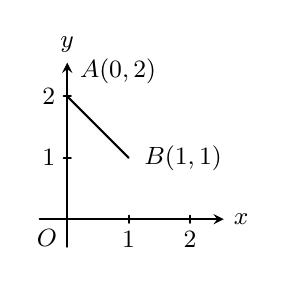
\begin{tikzpicture}[x=0.78cm,y=0.78cm,line cap=round,line join=round,line width=0.65pt,>=stealth,font=\small]
  \draw[->] (-0.45,0) -- (2.55,0) node[right] {$x$};
  \draw[->] (0,-0.45) -- (0,2.55) node[above] {$y$};
  \draw (-0.06,1) -- (0.06,1) node[left=2pt] {$1$};
  \draw (-0.06,2) -- (0.06,2) node[left=2pt] {$2$};
  \draw (1,-0.06) -- (1,0.06) node[below=2pt] {$1$};
  \draw (2,-0.06) -- (2,0.06) node[below=2pt] {$2$};
  \node[below left] at (0,0) {$O$};
  \draw[thick] (0,2) -- (1,1);
  \node[above right=1pt] at (0,2) {$A(0,2)$};
  \node[right=2pt] at (1,1) {$B(1,1)$};
\end{tikzpicture}
\end{center}
\nopagebreak[4]
\Needspace{4\baselineskip}
\textbf{解析}

\Needspace{5\baselineskip}
线段 $AB$ 的端点为 $A(0,2)$、$B(1,1)$，所以在 $[0,1]$ 上

\nopagebreak[4]
\[
f(t)=2-t.
\]

\Needspace{5\baselineskip}
当 $1\le x\le2$ 时，由周期为 $2$ 及偶函数性质，

\nopagebreak[4]
\[
f(x)=f(x-2)=f(2-x)=2-(2-x)=x.
\]

\gkanswer{答案：$f(x)=x$（$1\leq x\leq2$）}

\end{answer}
\begin{answer}
\gksolhead{9}{}

\textbf{题目}：

在二项式 $(x-1)^{11}$ 的展开式中，系数最小的项的系数为 $\underline{\qquad}$。（结果用数值表示）

\Needspace{4\baselineskip}
\textbf{解析}

\Needspace{5\baselineskip}
展开式通项为

\nopagebreak[4]
\[
(-1)^k\binom{11}{k}x^{11-k},\qquad 0\le k\le11.
\]

二项式系数最大值为 $\binom{11}{5}=\binom{11}{6}=462$。其中 $k=5$ 时系数为负，$k=6$ 时系数为正，因此最小系数为 $-462$。

\gkanswer{答案：$-462$}

\end{answer}
\begin{answer}
\gksolhead{10}{}

\textbf{题目}：

有红、黄、蓝三种颜色的旗帜各 3 面，在每种颜色的 3 面旗帜上分别标上号码 1、2 和 3。现任取出 3 面，它们的颜色与号码均不相同的概率是 $\underline{\qquad}$。

\Needspace{4\baselineskip}
\textbf{解析}

\Needspace{5\baselineskip}
9 面旗帜中任取 3 面共有

\nopagebreak[4]
\[
\binom93=84
\]

\Needspace{5\baselineskip}
种取法。颜色与号码均不相同，要求三种颜色各取一面，且 1、2、3 三个号码各出现一次；将三个号码分配给三种颜色有 $3!=6$ 种。因此所求概率为

\nopagebreak[4]
\[
\frac{6}{84}=\frac1{14}.
\]

\gkanswer{答案：$\dfrac{1}{14}$}

\end{answer}
\begin{answer}
\gksolhead{11}{}

\textbf{题目}：

\Needspace{5\baselineskip}
图中阴影部分的点满足不等式组

\nopagebreak[4]
\[
\begin{cases}
x+y\leq 5,\\
2x+y\leq 6,\\
x\geq 0,\quad y\geq 0,
\end{cases}
\]

在这些点中，使目标函数 $k=6x+8y$ 取得最大值的点的坐标是 $\underline{\qquad}$。
\nopagebreak[4]
\begin{center}% Source: src-8d14b1f9f511665ea10dbda45959a3b445a17806415be6b034f816bec663d7f5
% PDF SHA-256: 35e5d6f6bf052fcd9a2b91a1aa4215766fd4121425cfec7a62cfc4cdc7ab02a1
% PDF page 1, printed page 72, question 11. Shaded quadrilateral follows the printed inequalities.
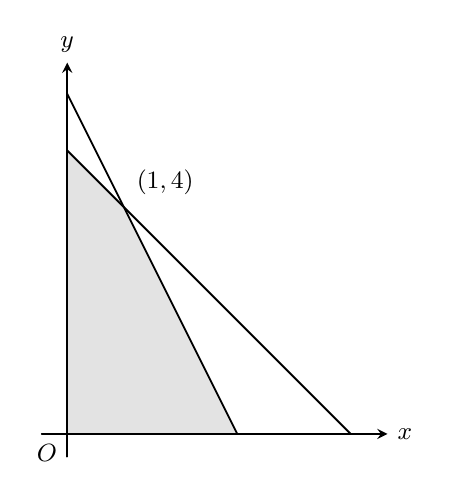
\begin{tikzpicture}[x=0.72cm,y=0.72cm,line cap=round,line join=round,line width=0.65pt,>=stealth,font=\small]
  \fill[gray!22] (0,0) -- (0,5) -- (1,4) -- (3,0) -- cycle;
  \draw[->] (-0.45,0) -- (5.65,0) node[right] {$x$};
  \draw[->] (0,-0.4) -- (0,6.55) node[above] {$y$};
  \draw (0,5) -- (5,0);
  \draw (0,6) -- (3,0);
  \node[below left] at (0,0) {$O$};
  \node[above right=1pt] at (1,4) {$(1,4)$};
\end{tikzpicture}
\end{center}
\nopagebreak[4]
\Needspace{4\baselineskip}
\textbf{解析}

\Needspace{5\baselineskip}
由不等式组和图示，闭可行域顶点为

\nopagebreak[4]
\[
(0,0),\quad(3,0),\quad(1,4),\quad(0,5).
\]

线性目标函数 $k=6x+8y$ 在多边形顶点处取得最大值。各顶点对应的函数值为 $0,18,38,40$，故最大值在 $(0,5)$ 处取得。图中标记的交点 $(1,4)$ 的目标值为 $38$，不是最大值点。

\gkanswer{答案：$(0,5)$}

\end{answer}
\begin{answer}
\gksolhead{12}{}

\textbf{题目}：

\Needspace{5\baselineskip}
在等差数列 $\{a_n\}$ 中，若 $a_{10}=0$，则有等式

\nopagebreak[4]
\[
a_1+a_2+\cdots+a_n=a_1+a_2+\cdots+a_{19-n}\quad(n<19,\ n\in\mathbb{N}^{*})
\]

成立。类比上述性质，相应地：在等比数列 $\{b_n\}$ 中，若 $b_9=1$，则有等式 $\underline{\qquad}$ 成立。

\Needspace{4\baselineskip}
\textbf{解析}

\Needspace{5\baselineskip}
设等比数列的公比为 $q$。由 $b_9=1$，有

\nopagebreak[4]
\[
b_j=q^{j-9}.
\]

\Needspace{5\baselineskip}
因 $b_9=1$，故 $q\ne0$。当 $1\le n<17$ 时，

\nopagebreak[4]
\[
b_1b_2\cdots b_n
=q^{\sum_{j=1}^{n}(j-9)}
=q^{n(n-17)/2}.
\]

\Needspace{5\baselineskip}
另一边有

\nopagebreak[4]
\[
b_1b_2\cdots b_{17-n}
=q^{\sum_{j=1}^{17-n}(j-9)}
=q^{(17-n)(-n)/2}
=q^{n(n-17)/2}.
\]

\Needspace{5\baselineskip}
故

\nopagebreak[4]
\[
b_1b_2\cdots b_n=b_1b_2\cdots b_{17-n}\qquad(1\le n<17).
\]

\gkanswer{答案：$b_1b_2\cdots b_n=b_1b_2\cdots b_{17-n}$（$1\leq n<17$）}

\end{answer}
\gkpart{二、选择题}

\begin{answer}
\gksolhead{13}{}

\textbf{题目}：

函数 $y=\sin\left(x+\dfrac{\pi}{2}\right)$（$\left[-\dfrac{\pi}{2},\dfrac{\pi}{2}\right]$）是\mbox{（　　）}。

（A）增函数　　（B）减函数　　（C）偶函数　　（D）奇函数

\Needspace{4\baselineskip}
\textbf{解析}

\nopagebreak[4]
\[
y=\sin\left(x+\frac\pi2\right)=\cos x.
\]

由于 $\cos(-x)=\cos x$，该函数在给定对称区间上为偶函数，选（C）。

\gkanswer{答案：C}

\end{answer}
\begin{answer}
\gksolhead{14}{}

\textbf{题目}：

设有不同的直线 $a$、$b$ 和不同的平面 $\alpha$、$\beta$、$\gamma$，给出下列三个命题：

① 若 $a\parallel\alpha$，$b\parallel\alpha$，则 $a\parallel b$；

② 若 $a\parallel\alpha$，$a\parallel\beta$，则 $\alpha\parallel\beta$；

③ 若 $\alpha\perp\gamma$，$\beta\perp\gamma$，则 $\alpha\parallel\beta$。

其中正确的个数是\mbox{（　　）}。

（A）0　　（B）1　　（C）2　　（D）3

\Needspace{4\baselineskip}
\textbf{解析}

三个命题均不成立，故正确命题有 $0$ 个，选（A）。

\Needspace{5\baselineskip}
① 两条直线可以同时平行于一个平面，却彼此相交。例如取平面 $z=0$，令

\nopagebreak[4]
\[
a=\{(t,0,1):t\in\mathbb R\},\qquad
b=\{(0,t,1):t\in\mathbb R\}.
\]

两线相交于 $(0,0,1)$，故不平行。

② 直线可以同时平行于两个相交平面。例如取 $\alpha:z=0$、$\beta:x=0$，令 $a=\{(1,t,1):t\in\mathbb R\}$。该直线与两平面都无交点且方向平行于两平面，但 $\alpha$、$\beta$ 相交。

③ 两个平面可以同时垂直于同一平面而彼此相交。例如 $\gamma:z=0$、$\alpha:x=0$、$\beta:y=0$，其中 $\alpha$、$\beta$ 都垂直于 $\gamma$，但沿 $z$ 轴相交。

\gkanswer{答案：A（正确命题个数为 0）}

\end{answer}
\begin{answer}
\gksolhead{15}{}

\textbf{题目}：

若集合 $S=\{y\mid y=3^x,\ x\in\mathbb{R}\}$，$T=\{y\mid y=x^2-1,\ x\in\mathbb{R}\}$，则 $S\cap T$ 是\mbox{（　　）}。

（A）$S$　　（B）$T$　　（C）$\varnothing$　　（D）有限集

\Needspace{4\baselineskip}
\textbf{解析}

\Needspace{5\baselineskip}
集合 $S$ 是 $3^x$ 的值域，故 $S=(0,+\infty)$；集合 $T$ 是 $x^2-1$ 的值域，故 $T=[-1,+\infty)$。因此

\nopagebreak[4]
\[
S\cap T=(0,+\infty)=S,
\]

选（A）。

\gkanswer{答案：A（$S$）}

\end{answer}
\begin{answer}
\gksolhead{16}{}

\textbf{题目}：

下列命题中正确的命题是\mbox{（　　）}。

（A）若点 $P(a,2a)$（$a\neq 0$）为角 $\alpha$ 终边上一点，则 $\sin\alpha=\dfrac{2\sqrt{5}}{5}$。

（B）同时满足 $\sin a=\dfrac{1}{2}$、$\cos a=\dfrac{\sqrt{3}}{2}$ 的角 $a$ 有且只有一个。

（C）当 $|a|<1$ 时，$\tan(\arcsin a)$ 的值恒正。

（D）三角方程 $\tan\left(x+\dfrac{\pi}{3}\right)=\sqrt{3}$ 的解集为 $\{x\mid x=k\pi,\ k\in\mathbb{Z}\}$。

\Needspace{4\baselineskip}
\textbf{解析}

选（D）。

\Needspace{5\baselineskip}
（A）点 $P(a,2a)$ 到原点的距离为 $\sqrt5|a|$，所以

\nopagebreak[4]
\[
\sin\alpha=\frac{2a}{\sqrt5|a|},
\]

该值随 $a$ 的正负变化，不恒等于题给的正值。

（B）同时满足两个三角方程的角为 $\alpha=\frac\pi6+2k\pi$，$k\in\mathbb Z$，不止一个。

\Needspace{5\baselineskip}
（C）在 $|a|<1$ 时

\nopagebreak[4]
\[
\tan(\arcsin a)=\frac{a}{\sqrt{1-a^2}},
\]

该值可以为负或为零，不恒正。

\Needspace{5\baselineskip}
（D）由正切函数的周期性，

\nopagebreak[4]
\[
x+\frac\pi3=\frac\pi3+k\pi,
\]

故 $x=k\pi$，与选项所给解集一致。

\gkanswer{答案：D}

\end{answer}
\gkpart{三、解答题}

\begin{answer}
\gksolhead{17}{}

\textbf{题目}：

已知椭圆 $C$ 的焦点分别为 $F_1(-2\sqrt{2},0)$ 和 $F_2(2\sqrt{2},0)$，长轴长为 6，设直线 $y=x+2$ 交椭圆 $C$ 于 $A$、$B$ 两点，求线段 $AB$ 的中点坐标。

\Needspace{4\baselineskip}
\textbf{解析}

\Needspace{5\baselineskip}
椭圆焦距参数为 $c=2\sqrt2$，长半轴为 $a=3$，因此

\nopagebreak[4]
\[
b^2=a^2-c^2=9-8=1,
\qquad
\frac{x^2}{9}+y^2=1.
\]

\Needspace{5\baselineskip}
代入直线 $y=x+2$，得

\nopagebreak[4]
\[
\frac{x^2}{9}+(x+2)^2=1
\quad\Longrightarrow\quad
10x^2+36x+27=0.
\]

\Needspace{5\baselineskip}
设交点横坐标为 $x_1,x_2$，则 $x_1+x_2=-\dfrac{18}{5}$。中点横坐标为 $-\dfrac95$；由直线方程，中点纵坐标为 $-\dfrac95+2=\dfrac15$。中点为

\nopagebreak[4]
\[
\left(-\frac95,\frac15\right).
\]

\gkanswer{答案：$\left(-\dfrac{9}{5},\dfrac{1}{5}\right)$}

\end{answer}
\begin{answer}
\gksolhead{18}{}

\textbf{题目}：

如图所示四面体 $ABCD$ 中，$AB$、$BC$、$BD$ 两两互相垂直，且 $AB=BC=2$，$E$ 是 $AC$ 中点，异面直线 $AD$ 与 $BE$ 所成的角的大小为 $\arccos\dfrac{\sqrt{10}}{10}$，求四面体 $ABCD$ 的体积。
\nopagebreak[4]
\begin{center}% Source: src-8d14b1f9f511665ea10dbda45959a3b445a17806415be6b034f816bec663d7f5
% PDF SHA-256: 35e5d6f6bf052fcd9a2b91a1aa4215766fd4121425cfec7a62cfc4cdc7ab02a1
% PDF page 1, printed page 72, question 18. Schematic topology only; no metric properties are inferred.
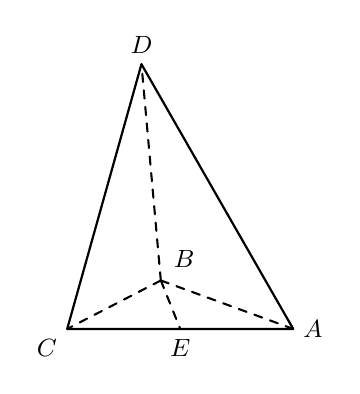
\begin{tikzpicture}[x=0.82cm,y=0.82cm,line cap=round,line join=round,line width=0.75pt,font=\small]
  \coordinate (A) at (3.5,0);
  \coordinate (B) at (1.45,0.75);
  \coordinate (C) at (0,0);
  \coordinate (D) at (1.15,4.1);
  \coordinate (E) at (1.75,0);
  \draw[thick] (C)--(D)--(A)--(C);
  \draw[dashed] (B)--(A) (B)--(C) (B)--(D) (B)--(E);
  \node[above] at (D) {$D$};
  \node[above right=1pt] at (B) {$B$};
  \node[below left] at (C) {$C$};
  \node[right] at (A) {$A$};
  \node[below] at (E) {$E$};
\end{tikzpicture}
\end{center}
\nopagebreak[4]
\Needspace{4\baselineskip}
\textbf{解析}

\Needspace{5\baselineskip}
取 $B=(0,0,0)$，令

\nopagebreak[4]
\[
A=(2,0,0),\qquad C=(0,2,0),\qquad D=(0,0,d),\quad d>0.
\]

\Needspace{5\baselineskip}
由 $E$ 是 $AC$ 中点，得 $E=(1,1,0)$。可取方向向量

\nopagebreak[4]
\[
\overrightarrow{AD}=(-2,0,d),\qquad \overrightarrow{BE}=(1,1,0).
\]

\Needspace{5\baselineskip}
异面直线所成角取锐角或直角，因此

\nopagebreak[4]
\[
\cos\angle(AD,BE)
=\frac{|\overrightarrow{AD}\cdot\overrightarrow{BE}|}
{|\overrightarrow{AD}|\,|\overrightarrow{BE}|}
=\frac{2}{\sqrt{d^2+4}\sqrt2}
=\frac{\sqrt{10}}{10}.
\]

\Needspace{5\baselineskip}
解得 $d=4$。又因 $BD\perp AB$ 且 $BD\perp BC$，而 $AB$、$BC$ 是平面 $ABC$ 内相交的两条直线，所以 $BD\perp$ 平面 $ABC$。底面面积 $S_{ABC}=\dfrac12\cdot2\cdot2=2$，高为 $BD=4$，故

\nopagebreak[4]
\[
V_{ABCD}=\frac13S_{ABC}\cdot BD=\frac13\cdot2\cdot4=\frac83.
\]

\gkanswer{答案：$\dfrac{8}{3}$}

\end{answer}
\begin{answer}
\gksolhead{19}{}

\textbf{题目}：

已知函数 $f(x)=\dfrac{x^2+2x+a}{x}$，$x\in[1,+\infty)$。

（1） 当 $a=\dfrac{1}{2}$ 时，求函数 $f(x)$ 的最小值；

（2） 若对任意 $x\in[1,+\infty)$，$f(x)>0$ 恒成立，试求实数 $a$ 的取值范围。

\Needspace{4\baselineskip}
\textbf{解析}

\Needspace{5\baselineskip}
将函数改写为

\nopagebreak[4]
\[
f(x)=x+2+\frac ax,\qquad x\ge1.
\]

\gksubpart{(1)}
\Needspace{5\baselineskip}
当 $a=\dfrac12$ 时，

\nopagebreak[4]
\[
f'(x)=1-\frac{1}{2x^2}>0\qquad(x\ge1),
\]

\Needspace{5\baselineskip}
故函数递增，最小值在 $x=1$ 处取得：

\nopagebreak[4]
\[
f(1)=1+2+\frac12=\frac72.
\]

\gksubpart{(2)}
\Needspace{5\baselineskip}
由于 $x\ge1$，分母 $x>0$，于是 $f(x)>0$ 等价于

\nopagebreak[4]
\[
x^2+2x+a>0\qquad(x\ge1).
\]

函数 $x^2+2x$ 在 $[1,+\infty)$ 上递增，最小值为 $3$。所以原不等式对定义域内所有 $x$ 严格成立，当且仅当 $3+a>0$，即 $a>-3$。

\gkanswer{答案（1）：$\dfrac{7}{2}$（在 $x=1$ 处取得）}

\gkanswer{答案（2）：$a>-3$}

\end{answer}
\begin{answer}
\gksolhead{20}{}

\textbf{题目}：

根据指令 $(r,\theta)$（$r\geq 0$，$-180^\circ\leq\theta\leq180^\circ$），机器人在平面上能完成下列动作：先原地旋转角度 $\theta$（$\theta$ 为正时，按逆时针方向旋转 $\theta$；$\theta$ 为负时，按顺时针方向旋转 $-\theta$），再朝其面对的方向沿直线行走距离 $r$。

（1） 现机器人在直角坐标系的坐标原点，且面对 $x$ 轴正方向，试给机器人下一个指令，使其移动到点 $(4,4)$；

（2） 机器人在完成该指令后，发现在点 $(17,0)$ 处有一小球正向坐标原点作匀速直线滚动。已知小球滚动的速度为机器人直线行走速度的 2 倍，若忽略机器人原地旋转所需的时间，问机器人最快可在何处截住小球？并给出机器人截住小球所需的指令。（结果精确到小数点后两位）
\nopagebreak[4]
\begin{center}% Source: src-8d14b1f9f511665ea10dbda45959a3b445a17806415be6b034f816bec663d7f5
% PDF SHA-256: 35e5d6f6bf052fcd9a2b91a1aa4215766fd4121425cfec7a62cfc4cdc7ab02a1
% PDF page 2, printed page 73, question 20. Only the coordinate axes and printed ticks are shown.
\begin{tikzpicture}[x=0.22cm,y=0.22cm,line cap=round,line join=round,line width=0.65pt,>=stealth,font=\small]
  \draw[->] (-1.4,0) -- (19.2,0) node[right] {$x$};
  \draw[->] (0,-1.2) -- (0,5.3) node[above] {$y$};
  \draw (4,-0.24) -- (4,0.24) node[below=3pt] {$4$};
  \draw (17,-0.24) -- (17,0.24) node[below=3pt] {$17$};
  \draw (-0.24,4) -- (0.24,4) node[left=3pt] {$4$};
  \node[below left] at (0,0) {$O$};
\end{tikzpicture}
\end{center}
\nopagebreak[4]
\Needspace{4\baselineskip}
\textbf{解析}

\gksubpart{(1)}
从原点移动到 $(4,4)$ 的距离为 $4\sqrt2$，方向角为 $45^\circ$，指令为 $(4\sqrt2,45^\circ)$。

\gksubpart{(2)}
\Needspace{5\baselineskip}
设机器人截球点为 $(x,0)$，其从 $(4,4)$ 行走的距离为 $s$。机器人速度记为 $v$，经过时间 $s/v$，小球移动距离为 $2s$，位置为 $(17-2s,0)$。要截住小球，须满足

\nopagebreak[4]
\[
s^2=(x-4)^2+16,\qquad x=17-2s.
\]

\Needspace{5\baselineskip}
代入得

\nopagebreak[4]
\[
(13-2s)^2+16=s^2,
\]

解得 $s=5$ 或 $s=\dfrac{37}{3}$。最快截球取较小的正根 $s=5$，故截点为 $(17-2\cdot5,0)=(7,0)$。从 $(4,4)$ 到 $(7,0)$ 的方向角为 $-\arctan(4/3)\approx-53.13^\circ$。机器人原朝向为 $45^\circ$，需顺时针转 $-53.13^\circ-45^\circ=-98.13^\circ$。所需指令为 $(5.00,-98.13^\circ)$。

\gkanswer{答案（1）：$(4\sqrt{2},45^\circ)$}

\gkanswer{答案（2）：在 $(7,0)$ 截住；截住指令为 $(5.00,-98.13^\circ)$}

\end{answer}
\begin{answer}
\gksolhead{21}{}

\textbf{题目}：

\Needspace{5\baselineskip}
在 $xOy$ 平面上有一点列 $P_1(a_1,b_1)$、$P_2(a_2,b_2)$、$\cdots$、$P_n(a_n,b_n)$、$\cdots$。对每个自然数 $n$，点 $P_n$ 位于函数

\nopagebreak[4]
\[
y=2000\left(\dfrac{a}{10}\right)^2\quad(0<a<10)
\]

的图象上，且点 $P_n$、点 $(n,0)$ 与点 $(n+1,0)$ 构成一个以 $P_n$ 为顶点的等腰三角形。

\begin{gktip}
\textbf{源文疑点（Q21）}：固定原页印式为 $y=2000\left(\dfrac{a}{10}\right)^2$，本稿照录。按字面该式不含 $x$，与“函数图象上”及后续序列条件的关系异常；在取得可靠同版证据前不改写指数，相关答案保持待核。
\end{gktip}

（1） 求点 $P_n$ 的纵坐标 $b_n$ 的表达式；

（2） 若对每个自然数 $n$，以 $b_n$、$b_{n+1}$、$b_{n+2}$ 为边长能构成一个三角形，求 $a$ 的取值范围；

（3） 设 $c_n=\lg(b_n)$（$n\in\mathbb{N}$）。若 $a$ 取（2）中确定的范围内的最小整数，问数列 $\{c_n\}$ 前多少项的和最大？试说明理由。

\Needspace{4\baselineskip}
\textbf{解析}

\textbf{U/PENDING：固定题面字面读法}

固定 PDF 印式为 $y=2000(a/10)^2$，不含 $x$。以下只按该字面式推导，不据旁证改写题面。令 $c=2000(a/10)^2>0$。以 $(n,0)$、$(n+1,0)$ 为底边端点，$P_n$ 到这两点距离相等，故 $a_n=n+\dfrac12$，且图象高度给出 $b_n=c$。

\gksubpart{(1) 固定印式字面读法}

\nopagebreak[4]
\[
b_n=2000(a/10)^2.
\]

\gksubpart{(2) 固定印式字面读法}
三个边长 $b_n,b_{n+1},b_{n+2}$ 均为同一正数 $c$，故构成等边三角形。题面范围内所有 $0<a<10$ 均满足条件。

\gksubpart{(3) 固定印式字面读法}
范围内的最小整数为 $a=1$，此时 $b_n=20$，所以 $c_n=\lg20>0$ 为常数。前 $m$ 项和为 $m\lg20$，随 $m$ 严格增加且无界，不存在使前若干项和最大的有限项数。这与题目设问不相容，不能作为预期答案。

\textbf{U/PENDING：若暂按指数 $x$ 读法的条件推导}

\Needspace{5\baselineskip}
以下是假设分支，不是对题面的改录，也不是已核实答案。若原意为 $y=2000(a/10)^x$，等腰条件给出 $a_n=n+\dfrac12$，从而

\nopagebreak[4]
\[
b_n=2000(a/10)^{n+1/2}.
\]

\gksubpart{指数式条件分支：第 (2) 问}
\Needspace{5\baselineskip}
令 $q=a/10$，则 $0<q<1$。三个边长与 $b_n$ 成比例，依次为 $1,q,q^2$；三角形条件等价于 $1<q+q^2$，即

\nopagebreak[4]
\[
5(\sqrt5-1)<a<10.
\]

范围内的最小整数为 $a=7$。

\gksubpart{指数式条件分支：第 (3) 问}
\Needspace{5\baselineskip}
若取 $a=7$，则 $c_n=\lg2000+(n+\dfrac12)\lg0.7$，是递减等差数列。并且

\nopagebreak[4]
\[
b_{20}=2000(0.7)^{20.5}\approx1.34>1,
\qquad
b_{21}=2000(0.7)^{21.5}\approx0.93<1.
\]

因此 $c_1,\ldots,c_{20}>0$，从 $c_{21}$ 起各项为负，前项和在第 $20$ 项达到最大。此分支与新浪同期答案/评分副本一致，但其来源链与官方身份未核，不能据此解决固定题面冲突。

\gkanswer{答案（1）：U/PENDING；按固定印式字面读得 $b_n=2000\left(\dfrac{a}{10}\right)^2$}

\gkanswer{答案（2）：U/PENDING；按固定印式字面读法，$0<a<10$ 均满足}

\gkanswer{答案（3）：U/PENDING；按固定印式字面读法不存在最大有限项数}

\end{answer}
\begin{answer}
\gksolhead{22}{}

\textbf{题目}：

已知复数 $z_0=1-mi$（$m>0$）、$z=x+yi$ 和 $\omega=x'+y'i$，其中 $x$、$y$、$x'$、$y'$ 均为实数，$i$ 为虚数单位，且对于任意复数 $z$，有 $\omega=\overline{z_0}\cdot\overline{z}$、$|\omega|=2|z|$。

（1） 试求 $m$ 的值，并分别写出 $x'$ 和 $y'$ 用 $x$、$y$ 表示的关系式；

（2） 将 $(x,y)$ 作为点 $P$ 的坐标，$(x',y')$ 作为点 $Q$ 的坐标，上述关系可以看作是坐标平面上点的一个变换：它将平面上的点 $P$ 变到这一平面上的点 $Q$。已知点 $P$ 经该变换后得到的点 $Q$ 的坐标为 $(\sqrt{3},2)$，试求点 $P$ 的坐标；

（3） 若直线 $y=kx$ 上的任一点经上述变换后得到的点仍在该直线上，试求 $k$ 的值。

\Needspace{4\baselineskip}
\textbf{解析}

\gksubpart{(1)}
\Needspace{5\baselineskip}
由

\nopagebreak[4]
\[
\omega=\overline{z_0}\,\overline z=(1+mi)(x-yi)
=(x+my)+(mx-y)i
\]

\Needspace{5\baselineskip}
以及 $|\omega|=|z_0||z|=2|z|$，得 $|z_0|=2$。于是 $1+m^2=4$，结合 $m>0$ 得 $m=\sqrt3$。比较实部、虚部：

\nopagebreak[4]
\[
x'=x+\sqrt3y,\qquad y'=\sqrt3x-y.
\]

\gksubpart{(2)}
\Needspace{5\baselineskip}
将 $x'=\sqrt3$、$y'=2$ 代入，得

\nopagebreak[4]
\[
x+\sqrt3y=\sqrt3,\qquad \sqrt3x-y=2.
\]

解得 $P$ 的坐标为 $\left(\dfrac{3\sqrt3}{4},\dfrac14\right)$。

\gksubpart{(3)}
\Needspace{5\baselineskip}
若直线 $y=kx$ 上任一点经变换后仍在该直线上，需满足 $y'=kx'$。代入变换关系得

\nopagebreak[4]
\[
\sqrt3x-kx=k(x+\sqrt3kx).
\]

\Needspace{5\baselineskip}
由于该关系须对任意 $x$ 成立，得到

\nopagebreak[4]
\[
\sqrt3-k=k+\sqrt3k^2,
\qquad
\sqrt3k^2+2k-\sqrt3=0.
\]

解得 $k=\dfrac1{\sqrt3}$ 或 $k=-\sqrt3$。

\gkanswer{答案（1）：$m=\sqrt{3}$，$x'=x+\sqrt{3}y$，$y'=\sqrt{3}x-y$}

\gkanswer{答案（2）：$\left(\dfrac{3\sqrt{3}}{4},\dfrac{1}{4}\right)$}

\gkanswer{答案（3）：$k=\dfrac{1}{\sqrt{3}}$ 或 $k=-\sqrt{3}$}

\end{answer}